\documentclass[tikz,border=5pt]{standalone}
\usepackage{amsmath}
\begin{document}
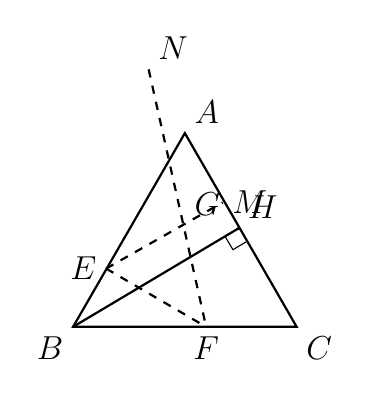
\begin{tikzpicture}[scale=1, font=\large]
  % Coordinates (in cm)
  \coordinate (A) at (2.22,2.46);
  \coordinate (B) at (0.80,0);
  \coordinate (C) at (3.64,0);
  \coordinate (M) at (2.70,1.58);
  \coordinate (E) at (1.22,0.74);
  \coordinate (F) at (2.49,0);
  \coordinate (G) at (2.22,1.29);
  \coordinate (N) at (1.76,3.27);
  \coordinate (H) at (2.90,1.25);

  % Triangle
  \draw[thick] (A) -- (B) -- (C) -- cycle;

  % Dashed auxiliary lines
  \draw[dashed, thick] (N) -- (F);
  \draw[dashed, thick] (E) -- (M);
  \draw[dashed, thick] (E) -- (F);

  % Perpendicular from B to line CM
  \draw[thick] (B) -- (H);

  % Right angle mark at H
  \draw[thin] (3.00,1.08) -- (2.83,0.98) -- (2.73,1.15);

  % Points
  \fill (H) circle (0.6pt);

  % Labels
  \node[above right] at (A) {$A$};
  \node[below left] at (B) {$B$};
  \node[below right] at (C) {$C$};
  \node[right] at (M) {$M$};
  \node[left] at (E) {$E$};
  \node[below] at (F) {$F$};
  \node[above right] at (G) {$G$};
  \node[above right] at (N) {$N$};
  \node[above right] at (H) {$H$};
\end{tikzpicture}
\end{document}
